% TeX root = ../../paper.tex

\section{Automatic Test Case Generation}\label{sec:automatically generates testcase}
\label{sec:generation}

The \emph{Petrinets Testing} language can automatically analyze the Petri net and automatically generate test cases of this petri net. We decided to use cause-effect-net \cite{Desel1997} to automatically create test cases. In this paper \cite{Desel1997}, the author introduced how to find Causes and Effects, and provided a method to create a casue-effect-net to generate a test case table. We adopt the method mentioned in the paper and implement it with a program to complete the automatic generation of the test case table about a given petri net.

\subsection{Test case generation}
We use the \emph{petrinets4analysis} language to parse the given Petri net and obtain the entire Petri net, and then use the algorithm to transform the Petri net into the cause-effect-net and get the test case table. \\

\begin{itemize}
    \item Step 1: Finding the causes and effects: \\
    First, finding all ALTERNATE-relationships in the given Petri net and recording the corresponding transitions. These transitions are the all non-determinism transition in the original Petri net and will be all transitions in the cause-effect-net. \\
    
    \item Step 2: Linking the causes and effects: \\
    Then analyzing all input places corresponding to these transitions using the OR-, AND-, SINGLE- and ALTERNATE-relationship and recording them. These associated input places are the causes. In addition, analyzing all output places corresponding to these transitions using the OR-, AND-, SINGLE- and ALTERNATE-relationship and recording them. These associated output places are the effects. \\
    
    \item Step 3: Generating cause-effect-net: \\
    According to the recorded transitions and the corresponding input and output places, a cause-effect-net of this Petri net can be created, which is similar to the generation of the Boolean graph. \\
    
    \item Step 4: Generating test case table: \\
    According to the generated cause-effect-net, each column in the test case table corresponds to a transition, and each row corresponds to the input and output places. When a transition has input and output places, the corresponding grid is marked as one.\\
    
    \item Step 5: Generating \emph{Petrinets Testing} model: \\
    According to the generated test case table, the simple transition test case model can be generated by the \emph{Petrinets Testing} language using PrettyPrinter. The test case model will be saved in the form of a file in the designated location to provide support for the next generating test code step.
    
\end{itemize}

\subsection{Example}
An specific example for the automatic test case generation from a Petri net, which is a simplified workflow of a cheap cookies machine (see Fig \ref{fig:cheap-cookie-machine}) with the following transitions:

First, coin is put into the cookies machine and will be checked whether is accepted. If the coin is accepted and the cookies button is pressed, the machine will receive the signal and give the cookies. At the same time, the amount of the cookies store and the number of cookies counter will be reduced. The machine will not accept a new signal until the money is cleared. \\

\begin{figure}
  \centering
  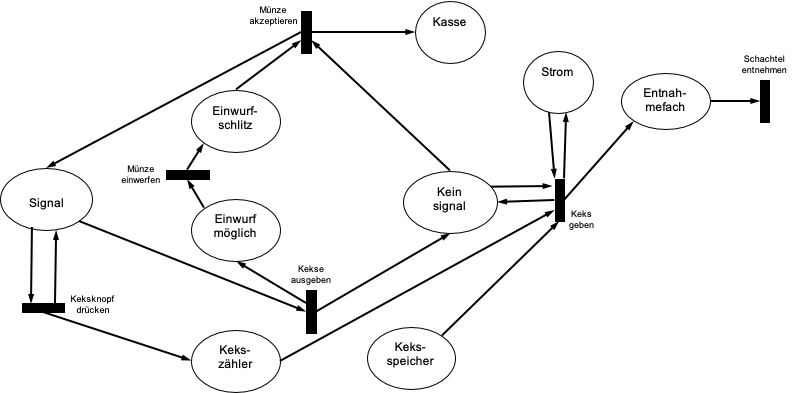
\includegraphics[scale=0.45]{src/pic/cheap-cookie-machine.png}
  \caption{Petri Net: Cheap Cookie Machine \cite{Hein}}
  \label{fig:cheap-cookie-machine}
\end{figure}

\subsubsection{Finding the causes and effects}
Firstly, we traverse all transitions in order to search all ALTERNATE-relationships in this Petri net. So we can find two places and four transitions that they meet the ALTERNATE-relationship conditions. They are \emph{Signal} places with \emph{Keksknopf drücken} and \emph{Kekse ausgeben} transitions, and \emph{Keinsignal} with \emph{Münze akzeptieren} and \emph{Keks geben} transitions. Then we record these four transitions into a temporary table.

\subsubsection{Linking the causes and effects}
Secondly, we analyze all input and output places about these four transitions using the OR-, AND-, SINGLE- and ALTERNATE-relationship and record them into a temporary table. The following is the temporary table about recorded transitions and input and output places:

\begin{enumerate}
    \item Transition: \emph{Keks drücken}
    \begin{itemize}
        \item Input places: \emph{Signal}
        \item Output places: \emph{Signal}, \emph{Kekszähler}
    \end{itemize}
    \item Transition: \emph{Kekse ausgeben}
    \begin{itemize}
        \item Input places: \emph{Signal}
        \item Output places: \emph{Einwurfmöglich}, \emph{Keinsignal}
    \end{itemize}
    \item Transition: \emph{Keks geben}
    \begin{itemize}
        \item Input places: \emph{Kekszähler}, \emph{Keksspeicher}, \emph{Strom}, \emph{Keinsignal}
        \item Output places: \emph{Keinsignal}, \emph{Entnahmefach}, \emph{Strom}
    \end{itemize}
    \item Transition: \emph{Münze akzeptieren}
    \begin{itemize}
        \item Input places: \emph{Keinsignal}, \emph{Einwurfschlitz}
        \item Output places: \emph{Kasse}
    \end{itemize}
\end{enumerate}

\subsubsection{Generating cause-effect-net}
According to the temporary table above, we can create a cause-effect-net (see Fig \ref{fig:cause-effect-net}) of the original Petri net. At the same time, we mark transition \emph{Keks drücken} as 1, taransition \emph{Kekse ausgeben} as 2, transition \emph{Keks geben} as 3 and transition \emph{Münze akzeptieren} as 4 for the convenience of generating test case table.

\begin{figure}
  \centering
  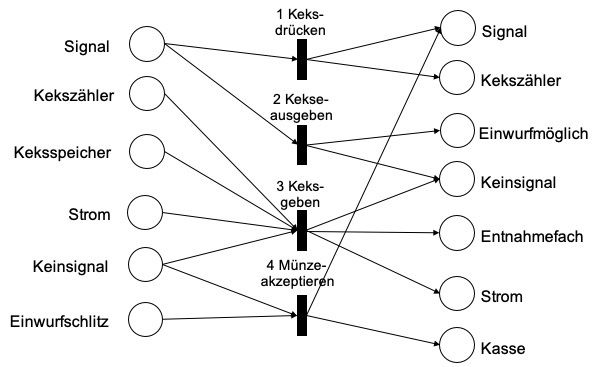
\includegraphics[scale=0.5]{src/pic/cause-effect-net.png}
  \caption{cause-effect-net of Cheap Cookie Machine model}
  \label{fig:cause-effect-net}
\end{figure}

\subsubsection{Generating test case table}
According to the cause-effect-net above, we can create a test case table (see Table \ref{tab:test-case-table}). In this table, we use the previously marked numbers 1,2,3,4 to represent transitions. In addition, Causes (Input places) and Effects (Output places) are distinguished. For example, we mainly focus on the third column in the table and the number 3 on the header stands for transition \emph{Keks geben}. Because \emph{Kekszähler}, \emph{Keksspeicher}, \emph{Strom}, \emph{Keinsignal} are the input places of transition \emph{Keks geben}, all corresponding positions in Causes are marked as 1. Similarly, \emph{Keinsignal}, \emph{Entnahmefach}, \emph{Strom} are the output places of transition \emph{Keks geben}, so all corresponding positions in Effects are marked as 1. Other transitions are marked by analogy. Finally we get a complete test case table about Petri net "Cheap Cookies Machine".

\begin{table}[]
    \centering
    \caption{Test case table of Cheap Cookie Machine model}
    \label{tab:test-case-table}
    \begin{tabular}{|p{3cm}|p{.5cm}<{\centering}|p{.5cm}<{\centering}|p{.5cm}<{\centering}|p{.5cm}<{\centering}|}
        \hline
        \rowcolor{gray} 
        \textbf{TestCase}   & 1  & 2  & 3  & 4  \\ \hline
        \multicolumn{5}{|l|}{\textbf{Causes:}}  \\ \hline
        Signal              & 1  & 1  & 0  & 0  \\ \hline
        Kekszähler          & 0  & 0  & 1  & 0  \\ \hline
        Keksspeicher        & 0  & 0  & 1  & 0  \\ \hline
        Strom               & 0  & 0  & 1  & 0  \\ \hline
        Keinsignal          & 0  & 0  & 1  & 1  \\ \hline
        Einwurfschlitz      & 0  & 0  & 0  & 1  \\ \hline
        \multicolumn{5}{|l|}{}                  \\ \hline
        \multicolumn{5}{|l|}{\textbf{Effects:}} \\ \hline
        Signal              & 1  & 0  & 0  & 1  \\ \hline
        Kekszähler          & 1  & 0  & 0  & 0  \\ \hline
        Einwurfmöglich      & 0  & 1  & 0  & 0  \\ \hline
        Keinsignal          & 0  & 1  & 1  & 0  \\ \hline
        Entnahmefach        & 0  & 0  & 1  & 0  \\ \hline
        Strom               & 0  & 0  & 1  & 0  \\ \hline
        Kasse               & 0  & 0  & 0  & 1  \\ \hline
    \end{tabular}
\end{table}

\subsubsection{Generating \emph{Petrinets Testing} model}
According to the test case table above, the program can automatically generate a \emph{Petrinets Testing} model about transition test. Each column in the test case table will generate a testcase in the \emph{Petrinets Testing} model. The corresponding Causes in the table will be used as \emph{initial marking} in the model. Moreover, the corresponding Effects in the table will be used as \emph{expect marking} in the model and the transition will be used as \emph{simulate} in the model. Then the program uses the PrettyPrinter of the \emph{Petrinets Testing} language to write the model into a file (see Listing \ref{lst:pnt-Cheap Cookie Machine}).

\begin{lstfloat}
	\centering
    \begin{lstlisting}[style=mcgrammar]
pntest CookieMachine_AutoTest { 
    use petrinet CookieMachine_modified
    testcase KeksGeben_TransitionTest {
        initial marking {
            KeksZaehler 1,
            Keksspeicher 1,
            KeinSignal 1,
            Strom 1
        }
        simulate {
            KeksGeben
        }
        expect marking {
            KeinSignal 1,
            Entnahmefach 1,
            Strom 1
        }
    }
    ...
}
    \end{lstlisting}
	\caption{The \emph{Petrinets Testing} model of Cheap Cookie Machine model}
	\label{lst:pnt-Cheap Cookie Machine}
\end{lstfloat}